% !TeX encoding = UTF-8
% !TeX root = ../main.tex

\section{CPS到SSA的转换算法}

\begin{frame}{PCF语言}
    \textcolor{DarkBlue}{本文研究的函数式编程语言是PCF(Programming Computable Functions)}。
    \begin{columns}[t, onlytextwidth]
        \column{0.5\textwidth}
        \begin{figure}
            \centering
            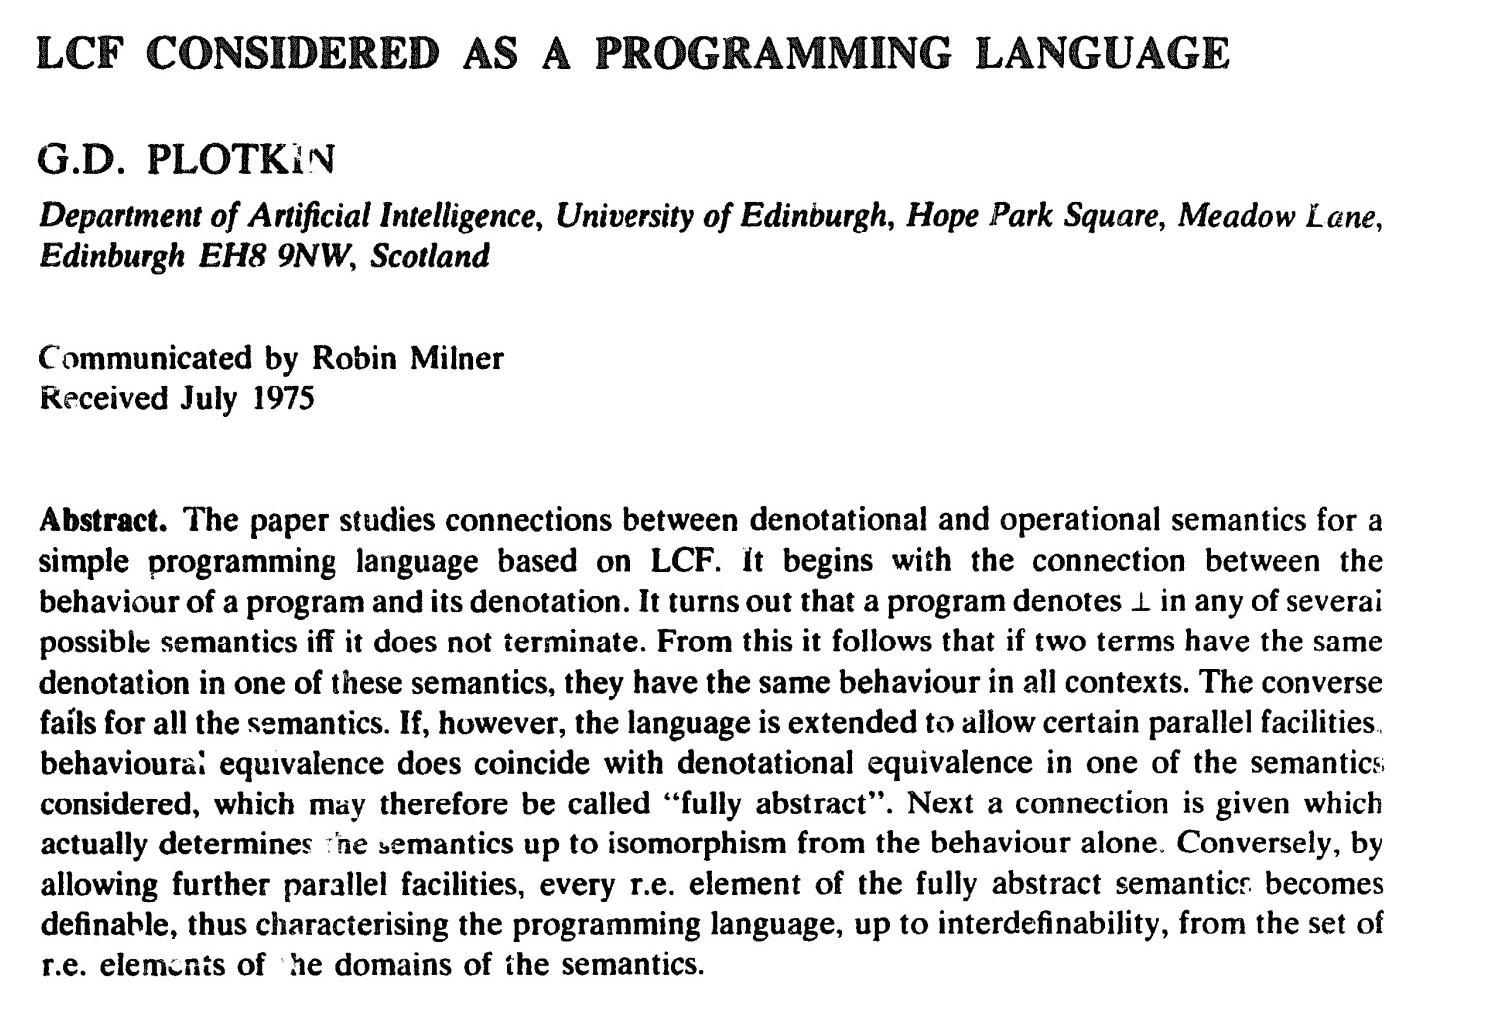
\includegraphics[width=\linewidth]{figures/pcf.jpg}
          \end{figure}
        \column{0.5\textwidth}
        \begin{itemize}
        \item PCF是学术界有广泛影响力的函数式语言。
        \item PCF可以看作是工业用函数式编程语言的核心。
        \item PCF是一种小规模的语言,但是能表示所有可计算的函数。
        \end{itemize}
    \end{columns}
\end{frame}

\begin{frame}
    \frametitle{源语言:CPS形式的PCF}
    \centering
    直接风格的PCF $\xrightarrow{\ \text{CPS转换}\ }$ \textcolor{Maroon}{CPS形式的PCF}
    \vspace{2ex}
    \begin{columns}[t, onlytextwidth]
     \column{0.5\textwidth}
        \textcolor{DarkBlue}{PCF语法}\\
        % \small
        $op\; := \; +\; |\; -\; | \; \times \; |\; \div$ \\
        $t\; := \; i\; |\; x\; |\; t_1\; t_2\; |\; \mathbf{ifz}\; t_1\; t_2\; t_3\; |\; op\; t_1\; t_2$ \\
        $\quad |\; \mathbf{let}\; x=t_1\; \mathbf{in}\; t_2 \; |\; \mathbf{fix}\; f\; x\; t$ \\
        % $\quad |\; \mathbf{let}\; x=t_1\; \mathbf{in}\; t_2$ \\
        \vspace{2ex}
        \normalsize
        \onslide<2>{
        \textcolor{DarkBlue}{CPS语法}\\
        % \small
        $v\; := \; i\; |\; x$ \\
        $t\; := \; \mathbf{letval}\; x=v\; \mathbf{in}\; t\; |\; k\; v\;  |\; f\; k\; v$\\
        $\quad |\;  \mathbf{ifz}\; v\; t_1\; t_2 \; |\; \mathbf{letcont}\; k\; x=t_1\; \mathbf{in}\; t_2$\\
        $\quad |\; \mathbf{letop}\; x=op\; x_1\; x_2\; \mathbf{in}\; t$ \\
        $\quad |\; \mathbf{letfun}\; f\; k\; x=t_1\; \mathbf{in}\; t_2 $
        } \\
      \column{0.5\textwidth}
        \textcolor{DarkBlue}{PCF示例程序}\\
        \vspace{1ex}
        % \small
        $(\mathbf{fix}\; f\; x\; =\; \mathbf{ifz}\; x\; 0\; 1) \ 2$ \\
        \vspace{2ex}
        \normalsize
        \onslide<2>{
        \textcolor{DarkBlue}{CPS示例程序}\\
        \vspace{1ex}
        % \small
        $\mathbf{letfun}\; f\; k\; x = (\mathbf{ifz}\; x$\\
        $\quad (\mathbf{letval}\; x_1=0\; \mathbf{in}\; k\; x_1)$\\
        $\quad (\mathbf{letval}\; x_2=1\; \mathbf{in}\; k\; x_2))\; \mathbf{in}$\\
        $(\mathbf{letval}\; x_3=2\; \mathbf{in}$\\
        $\quad  (\mathbf{letcont}\; k_2\; y=k_{init}\; y\; \mathbf{in}$\\
        $\quad\quad  (f\; k_2\; x_3)))$} \\
\end{columns}
\end{frame}

\begin{frame}
    \frametitle{目标SSA语言:简化版的LLVM IR}
    \begin{columns}[t, onlytextwidth]
    \column{0.4\textwidth}
    \textcolor{DarkBlue}{SSA语法}\\
    \vspace{1ex}
    % \small
    $t \coloneqq \overline{f}$ \\
    $  f \coloneqq \mathbf{define}\; l_1(l_2)\; \overline{b}$ \\
    $b \coloneqq l:\, \overline{\phi}\; \overline{a}\; r$ \\
    $a \coloneqq x = c;$ \\
    $ c \coloneqq v\; |\; op\; v_1\; v_2$\\
    $\quad\quad |\; \mathbf{icmp}\; v_1\; v_2\; |\; \mathbf{call}\; x\; v  $ \\
    \vspace{1ex}
    $ phi \coloneqq x = \phi \; \overline{(l,\; v)};$\\
    $r \coloneqq \mathbf{ret}\; v\; |\; \mathbf{br_{uc}}\; l\; |\; \mathbf{br_c}\; v\; l_1\; l_2$\\
    $  l \coloneqq string \quad  v \coloneqq i\; |\; x$\\
    
    \column{0.55\textwidth}
    \textcolor{DarkBlue}{SSA示例程序}\\
    \vspace{1ex}
    % \small
        $\mathbf{define}\; f\; (x)$\\
        $\quad b_1:\; b_0 = \mathbf{icmp}\; x\; 0;\; \mathbf{br_c}\; b_0\; t_0\; f_0;$ \\
        $\quad t_0:\; x_1 = 0;\; \mathbf{br_{uc}}\; if_0;$ \\
        $\quad f_0:\; x_2 = 1;\; \mathbf{br_{uc}}\; if_0;$\\
        $\quad if_0:\; r_x = \phi \; [(t_0,\, x_1),\, (f_0,\, x_2)];\; \mathbf{ret}\; r_x;$ \\
        \vspace{1ex}
        $\mathbf{define}\; main\; ( )$\\
        $\quad b_1:\; x_3 = 2;\; y = \mathbf{call}\; f\; x_3;\; \mathbf{br_{uc}}\; k_2;$\\
        $\quad k_2:\; r_{k2} = y;\; \mathbf{ret}\; r_{k2};$ \\
    \end{columns}
\end{frame}

\begin{frame}
    \frametitle{CPS到SSA的转换算法}
    \begin{columns}[t, onlytextwidth]
        \column{0.5\textwidth}
        \large
        \textcolor{DarkBlue}{找出结构上的对应关系:}\\
        \normalsize
        \vspace{2ex}
        \begin{columns}[t, onlytextwidth]
            \column{0.45\textwidth}
            \textcolor{Maroon}{CPS} \\
            \vspace{1ex}
            变量绑定 \\
            延续体 \\
            同一延续应用到\\ 不同的值上 \\
            ...
            \column{0.1\textwidth}
            \\
            \vspace{1ex}
            $\Rightarrow $ \\
            $\Rightarrow $ \\
            \vspace{1.5ex}
            $\Rightarrow $ \\
            \column{0.45\textwidth}
            \textcolor{Maroon}{SSA}\\
            \vspace{1ex}
            变量赋值\\
            新的基本代码块 \\
            \vspace{1.5ex}
            $\Phi$-节点 \\
        \end{columns}

    \column{0.5\textwidth}
    \large
    \textcolor{DarkBlue}{$\mathcal{G}$:递归转换函数}
    \normalsize
    \vspace{1ex}
    \begin{enumerate}
        \item \textcolor{Maroon}{初始:} $\mathcal{G}$读入待转换的CPS程序和空的SSA程序。
        \item \textcolor{Maroon}{递归翻译CPS程序:}
        \begin{itemize}
            \item 将新的组件(基本代码块、指令等)放入当前 SSA 程序的特定位置。
            \item 更新参数。
        \end{itemize}
        \item \textcolor{Maroon}{完成:} 返回当前SSA程序。  
    \end{enumerate}
\end{columns}
\end{frame}

\begin{frame}
    \frametitle{CPS到SSA的转换示例}

    \begin{columns}[t, onlytextwidth]
        \column{0.4\textwidth}
        \textcolor{DarkBlue}{CPS程序}\\
        \vspace{1ex}
        % \small
        $\mathbf{letfun}\; f\; \textcolor{DarkViolet}{k}\; x = (\mathbf{ifz}\; x$\\
        $\quad (\mathbf{letval}\; \textcolor{DarkViolet}{x_1}=0\; \mathbf{in}\; \textcolor{Brown}{k\; x_1})$\\
        $\quad (\mathbf{letval}\; \textcolor{DarkViolet}{x_2}=1\; \mathbf{in}\; \textcolor{Brown}{k\; x_2}))\; \mathbf{in}$\\
        $(\mathbf{letval}\; \textcolor{DarkViolet}{x_3}=2\; \mathbf{in}$\\
        $\quad  (\mathbf{letcont}\; \textcolor{DarkViolet}{k_2\; y}=k_{init}\; y\; \mathbf{in}$\\
        $\quad\quad  (f\; k_2\; x_3)))$ \\
        \hspace{2ex}
        \column{0.6\textwidth}
        \textcolor{DarkBlue}{转换得到的SSA程序}\\
        \vspace{1ex}
        % \small
        $\mathbf{define}\; f\; (x)$\\
        $\quad b_1:\; \textcolor{DarkViolet}{b_0} = \mathbf{icmp}\; x\; 0;\; \mathbf{br_c}\; b_0\; t_0\; f_0;$ \\
        $\quad t_0:\; x_1 = 0;\; \mathbf{br_{uc}}\; if_0;$ \\
        $\quad f_0:\; x_2 = 1;\; \mathbf{br_{uc}}\; if_0;$\\
        $\quad if_0:\; \textcolor{DarkViolet}{r_x} = \textcolor{Brown}{[(t_0,\, x_1),\, (f_0,\, x_2)]};\; \mathbf{ret}\; r_x;$ \\
        \vspace{1ex}
        $\mathbf{define}\; main\; ( )$\\
        $\quad b_1:\; x_3 = 2;\; y = \mathbf{call}\; f\; x_3;\; \mathbf{br_{uc}}\; k_2;$\\
        $\quad k_2:\; \textcolor{DarkViolet}{r_{k2}} = y;\; \mathbf{ret}\; r_{k2};$ \\
    \end{columns}
    % \vspace{1ex}
    \textcolor{Maroon}{可以观察到:} 
    \begin{itemize}
        \item 延续在不同位置应用,将控制流合并,表示需要插入$\Phi$-节点。
        \item 生成新变量的机制确保每个变量只被赋值一次。
    \end{itemize}
\end{frame}